% Build: cd figures && tectonic mips_task_examples_explained.tex
\documentclass[10pt]{article}
\usepackage[landscape,margin=0.6in]{geometry}
\usepackage{amsmath,amssymb,booktabs,graphicx,parskip}
\usepackage[hidelinks]{hyperref}
\newcommand{\op}[1]{\mathrm{#1}}
\title{Decoding the MIPS-evolved programs:\\Parity-last 4, Alternating-last 4, Base-4/5/7 addition}
\date{November 2, 2026}
\author{}
\begin{document}
\maketitle
\vspace{-2em}

\section*{Notation}
In every table, $h=(h_0,h_1,\ldots)$ is the RNN hidden state after mapping onto its learned
integer lattice; primes denote the next state; $x$ (or the digit pair $a,b$) is the
current input; and $y$ is the output read from the new state. Operators:
$\op{lt}(u,v)=\mathbf 1[u<v]$, $\op{eq}(u,v)=\mathbf 1[|u-v|<0.5]$,
$\op{zero}(u)=\op{not}(u)=\mathbf 1[|u|<0.5]$, $\op{mod}(u,v)=u\bmod|v|$ (0 if $v=0$),
$\op{xor}(u,v)=(\op{round}(u)+\op{round}(v))\bmod 2$.
Displayed equations are regrouped/rounded MIPS-evolved witnesses, verified exactly on the full
recorded transition tables. The state meanings below were obtained by labeling each
lattice state with the input histories that reach it.

%======================================================================
\clearpage
\section{Parity-last 4}
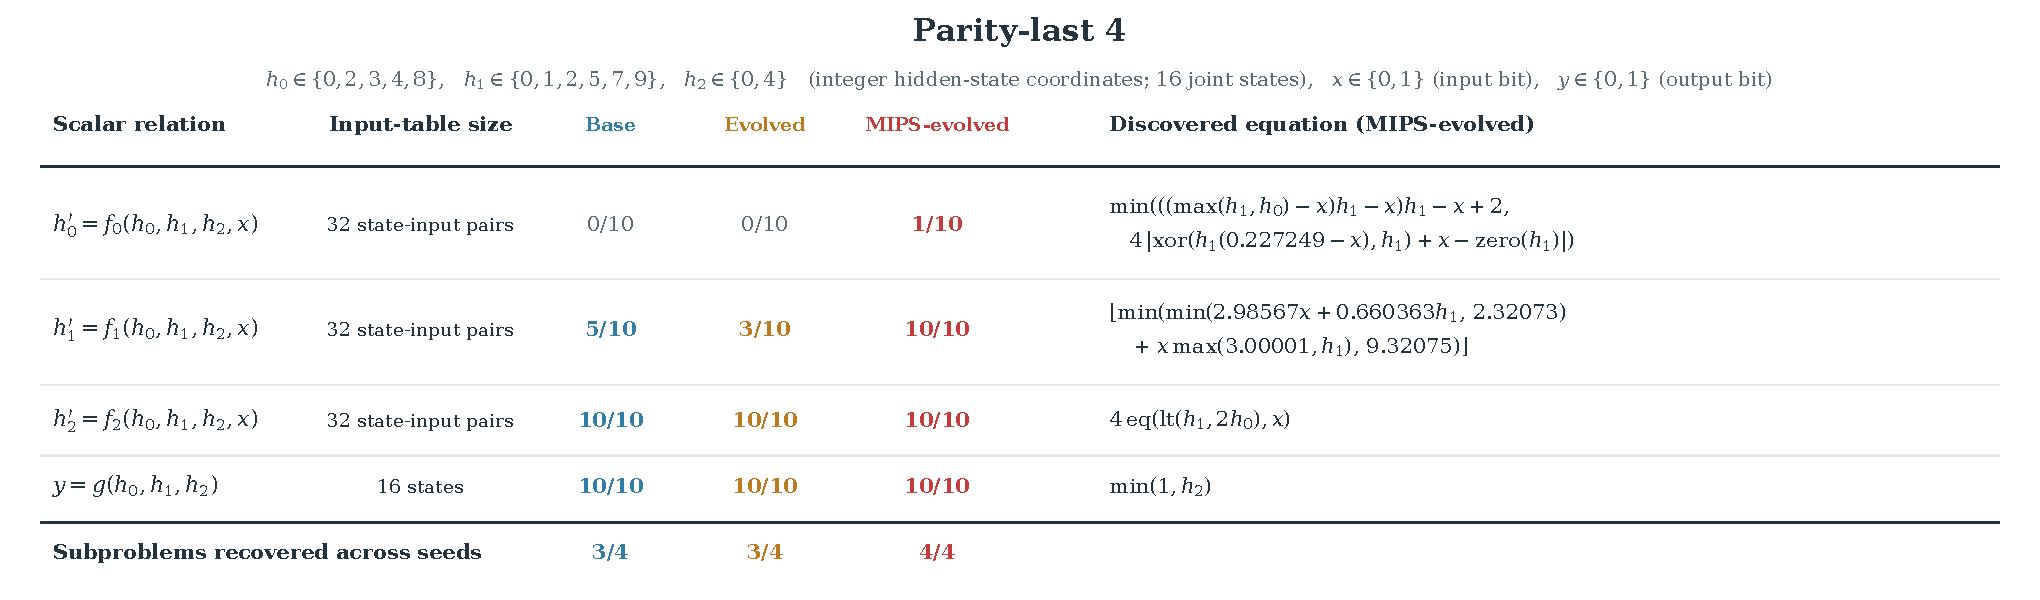
\includegraphics[width=\textwidth]{mips_parity_last4_example.pdf}

\textbf{Task.} $y_t$ = parity of the last 4 input bits.

\textbf{What the state stores.} 16 states $=$ all 4-bit windows $d\,a\,b\,c$ (oldest$\to$newest).
\begin{itemize}
\item $h_2 = 4\cdot$ parity of the 4-bit window, hence $y=\min(1,h_2)=h_2/4$.
\item $(h_0,h_1)$ is a shift register of the last 3 bits $a\,b\,c$:
\[
\begin{array}{c|cccccccc}
abc & 000 & 100 & 010 & 110 & 001 & 101 & 011 & 111\\\hline
(h_0,h_1) & (2|3,0) & (0,1) & (0,2) & (4,2) & (0,5) & (3|4,5) & (8,7) & (4,9)
\end{array}
\]
($2|3$ and $3|4$: small RNN noise that depends on the bit just dropped.)
\item $h_1$ essentially encodes the last two bits $(b,c)$: $\{0,1\}\!=\!00$, $2\!=\!10$, $5\!=\!01$, $\{7,9\}\!=\!11$,
roughly $h_1\approx 5c+2b+a$.
\end{itemize}

\textbf{Parity rule ($h_2'$) --- the real algorithm.} The new window is $a\,b\,c\,x$, so
new parity $=\op{parity}(a,b,c)\oplus x$, independent of the old $h_2$. On this embedding the
3-bit parity is \emph{linearly separable}: $h_1<2h_0 \iff \op{parity}(a,b,c)=0$ (true on all 10
distinct $(h_0,h_1)$). Then $\op{eq}(\cdot,x)$ is XNOR, giving $4\,(\op{parity}\oplus x)$.

\textbf{Shift of $h_1$.} The $2.98567x$ term is dead (the inner $\min$ saturates when $x=1$). Effectively
\[
h_1'=\begin{cases}\lfloor\min(0.66h_1,2.32)\rfloor: & \{0,1\}\to0,\;2\to1,\;\{5,7,9\}\to2 \quad (x=0)\\
\lfloor\min(2.32+\max(3,h_1),9.32)\rfloor: & h_1\le3\to5,\;5\to7,\;\{7,9\}\to9 \quad (x=1),\end{cases}
\]
i.e.\ shift the 2-bit code left and push in $x$.

\textbf{Shift of $h_0$ (least structured).} $h_0$'s target values have no clean bit pattern,
and the expression acts as a lookup table: the cubic $P$ in $h_1$ is huge unless $h_1\in\{0,1\}$
(and handles the single case where $h_0'$ depends on $h_0$, via $\max(h_1,h_0)$); $Q$ supplies
$\{0,4,8\}$ for $h_1\ge2$, with $0.227$ tuned so the rounded products have the right parity.
This is the subproblem the other methods miss.

%======================================================================
\clearpage
\section{Alternating-last 4}
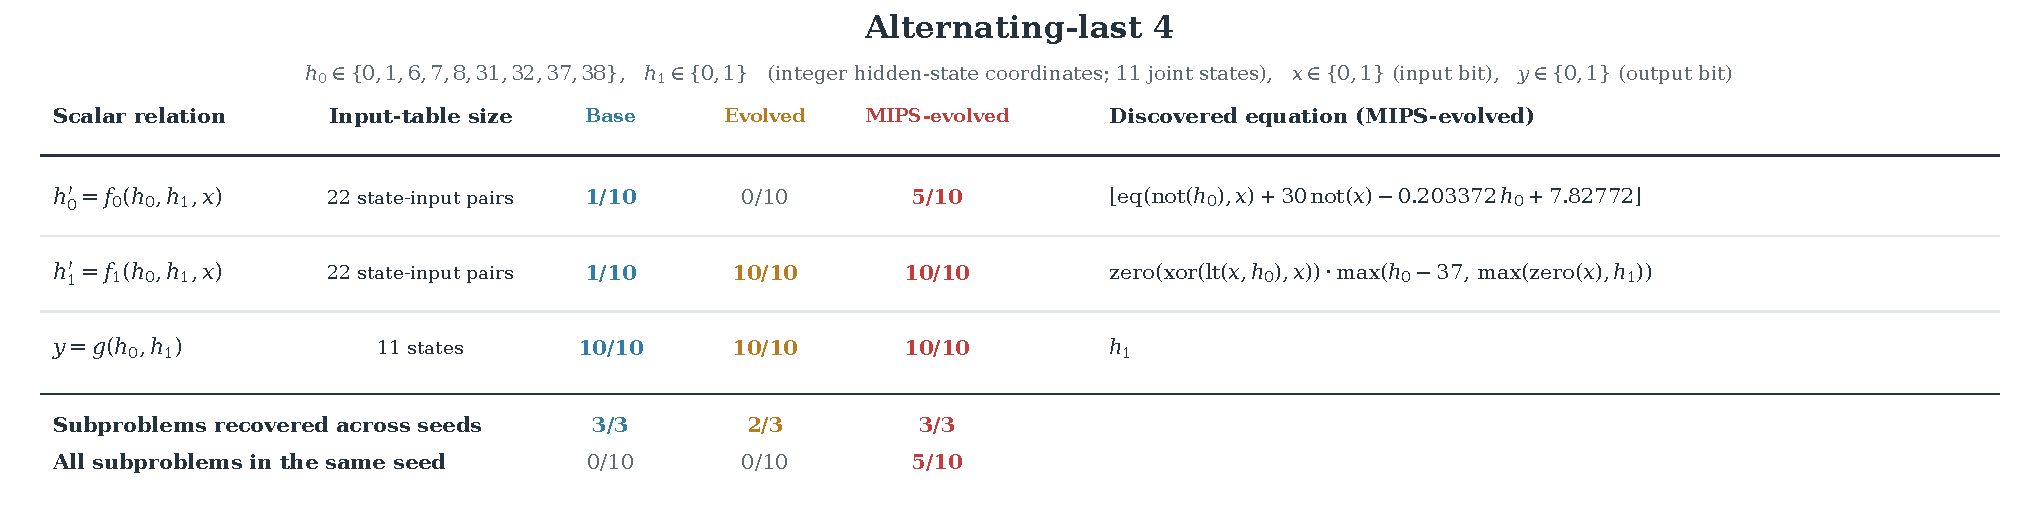
\includegraphics[width=\textwidth]{mips_alternating_last4_example.pdf}

\textbf{Task.} $y=1$ iff the last 4 bits alternate (0101 or 1010).

\textbf{What the state stores.} The last bit and the length $L$ of the current alternating run:
\[
\begin{array}{c|ccc|cccc}
h_0 & 6,7,8 & 1 & 0 & 31,32 & 37\,(h_1{=}0) & 38 & 37\,(h_1{=}1)\\\hline
\text{last bit} & 1&1&1 & 0&0&0&0\\
L & 1 & 2 & \ge3 & 1 & 2 & 3 & \ge4
\end{array}
\]
Small $h_0$ $\Leftrightarrow$ last bit 1; large $h_0$ (31--38) $\Leftrightarrow$ last bit 0.
$6,7,8$ and $31,32$ are redundant copies with identical transitions.
$h_1=\mathbf 1[L\ge4]$, so $y=h_1$.

\textbf{$h_0'$: an affine ``flip'' map.} Up to the small $\op{eq}$ term,
$h_0'\approx\lfloor 7.83-h_0/5+30\,\mathbf 1[x{=}0]\rfloor$.
\begin{itemize}
\item $x=1$: large $h_0$ (run continues) $\to$ small: $31/32\to1$ ($L{=}2$), $37/38\to0$ ($L{\ge}3$);
small $h_0$ (repeat, run resets) $\to6/7/8$ ($L{=}1$).
\item $x=0$: $+30$ lands in the large band: large $h_0$ (repeat) $\to31/32$; $6/7/8\to37$ ($L{=}2$),
$1\to38$ ($L{=}3$). The $\op{eq}(\op{not}(h_0),x)$ term is the $\pm1$ correction for $h_0=0$
($L{\ge}3\to37$ with $h_1'=1$).
\end{itemize}

\textbf{$h_1'$: ``run was already $\ge3$ and this bit continues it''.}
$\op{zero}(\op{xor}(\op{lt}(x,h_0),x))=1$ iff ($x{=}0$ and $h_0{=}0$) or ($x{=}1$ and $h_0\ge2$);
then $\max(h_0-37,\max(\op{zero}(x),h_1))$ keeps only the $L\ge3$ states ($h_0=0$; or
$h_0=38$ or $(37,h_1{=}1)$). $h_1$ is needed because $h_0=37$ alone does not separate $L=2$ from $L\ge4$.

%======================================================================
\clearpage
\section{Base-$B$ addition: shared structure}
\textbf{Task.} Each step reads one digit $a,b$ of two base-$B$ numbers (least significant first)
and outputs the corresponding digit of the sum.

\textbf{What the state stores.} The full column sum $s=a+b+c_{\text{in}}\in\{0,\ldots,2B-1\}$
($2B$ states: 8, 10, 14), as two coordinates: a \emph{carry bit} $\mathbf 1[s\ge B]$ and a
\emph{digit coordinate} that decreases in $s$ with a jump at the carry:
\[
\begin{array}{c|c|c}
B & \text{carry} & \text{digit coordinate}\\\hline
4 & h_1 & h_0 = 5-s+2h_1\\
5 & h_1 & h_0 = 6-s+3h_1\\
7 & h_0 & h_1 = 8-s+5h_0
\end{array}
\]
\textbf{Output} $y=s\bmod B$: invert the digit coordinate and subtract $B$ if the carry is set.
\textbf{Carry update} $c'=\mathbf 1[a+b+c\ge B]$: a threshold on $a+b$ plus carry.
\textbf{Digit update}: compute $K-s'+\delta\,\mathbf 1[s'\ge B]$ with $s'=a+b+c$, always as a
$\max/\min$ of a \emph{linear branch} ($s'<B$) and a \emph{mod branch} that implements the
``subtract $B$'' wrap-around.

%======================================================================
\clearpage
\section{Base-4 addition}
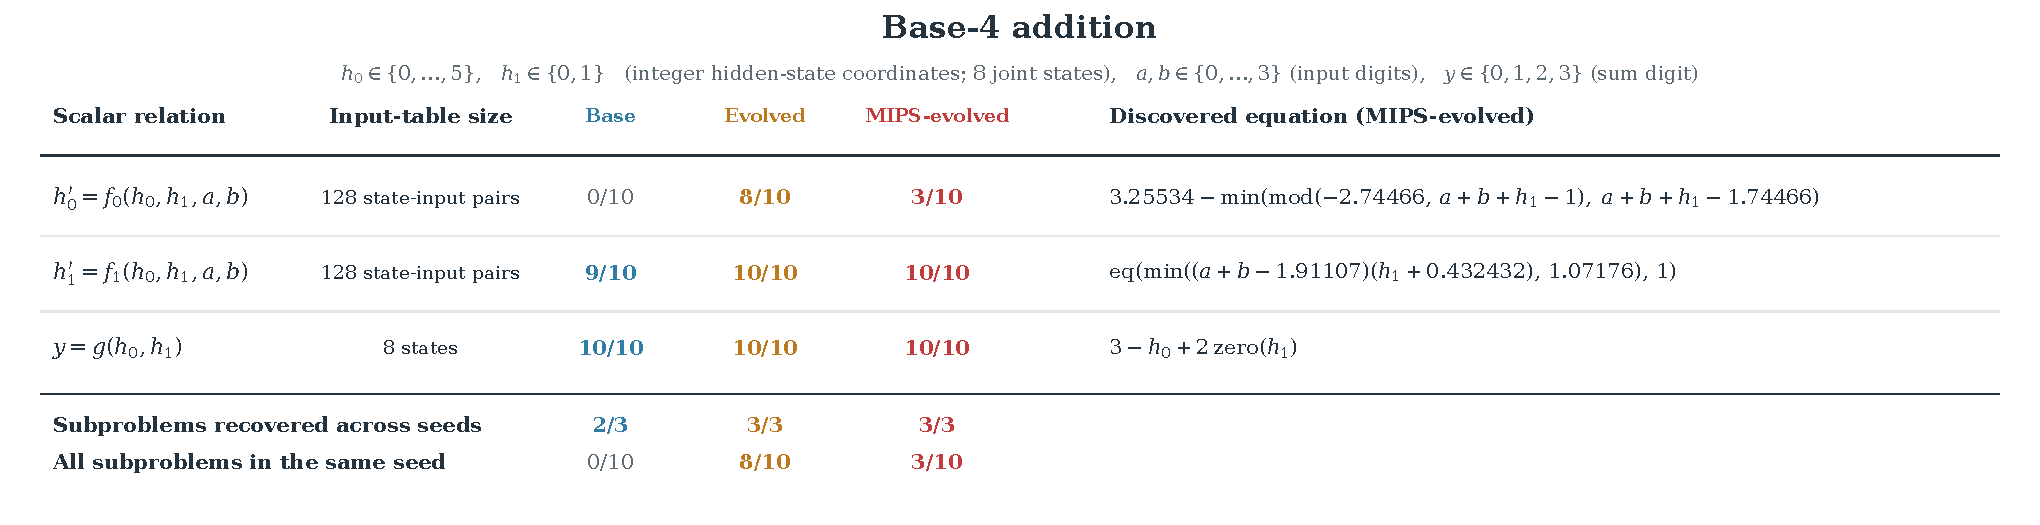
\includegraphics[width=\textwidth]{mips_base4_addition_example.pdf}

Carry $=h_1$, digit coordinate $h_0=5-s+2h_1$ ($s=0..3\mapsto5,4,3,2$; $s=4..7\mapsto3,2,1,0$).

\textbf{Output.} $y=3-h_0+2\,\op{zero}(h_1)$: no carry gives $3-(5-s)+2=s$; carry gives $3-(7-s)=s-4$.

\textbf{Carry.} $\op{eq}(\min((a{+}b{-}1.91)(h_1{+}0.43),1.07),1)$ fires iff $(a{+}b{-}1.91)(h_1{+}0.43)>0.5$:
with $h_1=0$ this needs $a{+}b>3.07$ ($\ge4$); with $h_1=1$, $a{+}b>2.26$ ($\ge3$). That is
$a+b+c\ge4$, with the carry changing the slope rather than the offset.

\textbf{Digit.} With $s'=a+b+h_1$: $3.255-\min(\op{mod}(-2.745,s'-1),\,s'-1.745)$.
Linear branch gives $5-s'$ for $s'<4$. For $s'\ge4$, $\op{mod}(-2.745,s'-1)=s'-3.745$, giving
$7-s'$ (the wrapped code). At $s'=2,3$ the two branches tie exactly.

%======================================================================
\clearpage
\section{Base-5 addition}
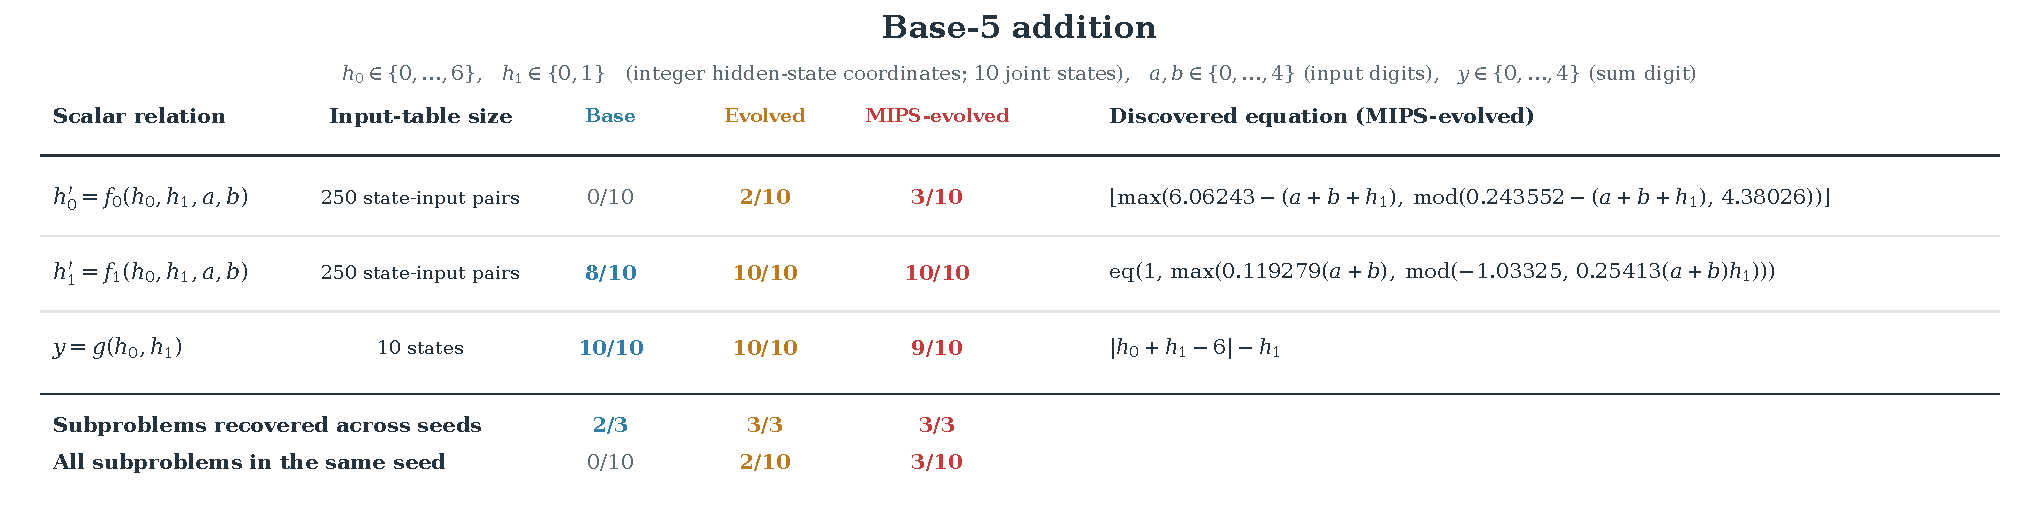
\includegraphics[width=\textwidth]{mips_base5_addition_example.pdf}

Carry $=h_1$, digit coordinate $h_0=6-s+3h_1$ ($s=0..4\mapsto6..2$; $s=5..9\mapsto4..0$).

\textbf{Output.} $y=|h_0+h_1-6|-h_1$: no carry gives $|-s|=s$; carry gives $|4-s|-1=s-5$.

\textbf{Carry.} $\op{eq}(1,\max(0.119(a{+}b),\op{mod}(-1.033,0.254(a{+}b)h_1)))$. Without carry the
mod term is 0 and $0.119(a{+}b)\in(0.5,1.5)$ iff $a{+}b\ge5$. With carry, the mod term lands at
$\approx1.0$ for $a{+}b=4$ and at $0.49$ (just under the 0.5 cutoff) for $a{+}b\le3$. Correct,
but a fragile modular coincidence.

\textbf{Digit.} With $s'=a+b+h_1$: $\lfloor\max(6.06-s',\,\op{mod}(0.24-s',4.38))\rfloor$.
For $s'\ge5$, two periods ($8.76$) give $\op{mod}\approx9-s'$, the wrapped code; otherwise
$6.06-s'$ dominates.

%======================================================================
\clearpage
\section{Base-7 addition}
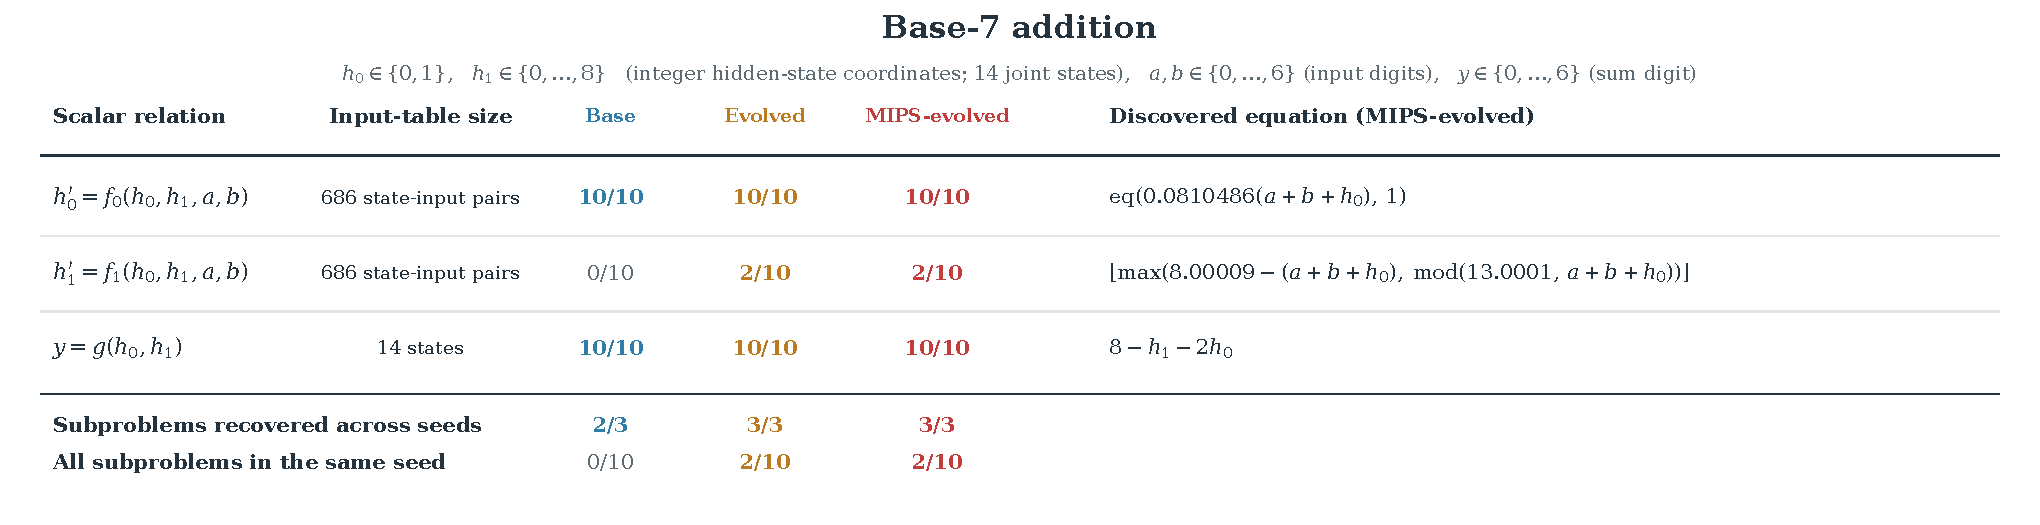
\includegraphics[width=\textwidth]{mips_base7_addition_example.pdf}

Roles swap: carry $=h_0$, digit coordinate $h_1=8-s+5h_0$ ($s=0..6\mapsto8..2$; $s=7..13\mapsto6..0$).

\textbf{Output.} $y=8-h_1-2h_0$: $s$ or $s-7$.

\textbf{Carry.} $\op{eq}(0.081(a+b+h_0),1)=1$ iff $a+b+h_0\in(6.2,18.5)$, i.e.\ exactly
$a+b+c\ge7$. The cleanest carry of the three.

\textbf{Digit.} $\lfloor\max(8-s',\,\op{mod}(13,s'))\rfloor$ with $s'=a+b+h_0$. For $s'\ge7$,
$13/s'<2$ so $\op{mod}(13,s')=13-s'$, the wrapped code; for $s'<7$ the mod value is below $8-s'$.
So $\op{mod}$ is used as a ``subtract once if large'' operator.

%======================================================================
\section*{Takeaways}
\begin{itemize}
\item The RNN representations are genuine algorithms: a shift register plus a running parity
(parity), last bit plus run length (alternating), and column sum as (carry, reversed digit)
(addition).
\item Clean, interpretable recoveries: the parity rule $h_1<2h_0$, all outputs, and the
base-4/base-7 carry thresholds.
\item The remaining coordinates (parity $h_0$, alternating $h_0$/$h_1$, digit updates, base-5
carry) are correct piecewise lookups built from $\lfloor\cdot\rfloor$, mod and max, often exploiting
numerical coincidences or the RNN's arbitrary, partly redundant lattice coordinates.
These are exactly the subproblems baseline and SRBench-evolved PySR tend to miss.
\end{itemize}
\end{document}
